
\chapter{Marco Teórico}
% En este capítulo, se presenta las principales tecnologías de detección en primer  plano del objeto en movimiento, descripción y extracción de características,  clasificación y reconocimiento del movimiento humano. Basado en el flujo óptico para la detección de objetos en movimiento. Como también la imagen de flujo de energía óptico para la detección de características de movimiento y se adoptaron redes neuronales convolucionales de región para elegir  características y reducir la dimensión. Luego, gracias al clasificador de máquina de vectores de soporte que puede ser entrenado y utilizado para clasificar y reconocer acciones; es posible distinguir efectivamente las acciones humanas y mejorar significativamente la precision del reconocimineto de las acciones humanas.

\section{Sistema de video vigilancia}
El término ``video-vigilancia'' es usado para hacer referencia al despliegue de cámaras de vídeo que cumplen el rol de videofilmadoras, las cuales guardan el contenido recolectado en un almacén digital y puede ser visualizado en un monitor central \cite{wikipedia:vvigilancia}. Por lo tanto, un sistema de video-vigilancia consiste en una instalación de seguridad cuya finalidad es el control y supervisión visual en tiempo real de instalaciones locales y remotas, mediante el uso de múltiples cámaras de vigilancia, así como de sistemas de visualización, grabación y archivo. Estos sistemas ayudan a proteger a las personas, bienes y recursos, manteniendo una alerta activa con un gran efecto disuasorio.\\

El sistema llega a capturar imágenes y vídeos, que pueden ser comprimidos, almacenados, o enviados por una red de comunicación y pueden ser instalados en cualquier ambiente. En la figura \ref{fig:sistema_video_vigilancia} se visualiza el conjunto de elementos que forman un sistema de video-vigilancia. Este sistema compone de un conjunto de cámaras que estan conectadas directamente a un grabador de video en red o N.V.R. (Network Video Recorder), el cual permite la visualización de las imágenes captadas por las cámaras en un monitor local y por medio de una conección a internet, permite su visualización en dispositivos externos a la red local.\\

\begin{figure}[H]
    \begin{center}
        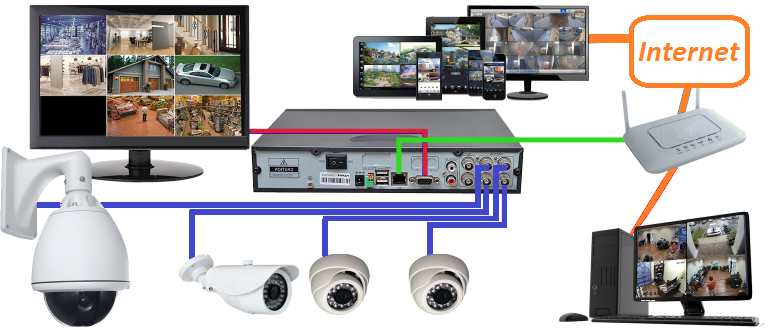
\includegraphics[width=7cm]{img/capitulo_2/sis_videovigilancia.png}
        \caption{Componentes de una sistema de video-vigilancia.\\}
        Fuente: \cite{videosurvellance}
        \label{fig:sistema_video_vigilancia}
    \end{center}
    
\end{figure}

Existe una amplia oportunidad para el mercado de la video-vigilancia en todas las regiones del mundo especialmente en Asia y la región del Pacífico, debido a la apertura de pequeños negocios y la construcción de áreas residenciales como también ciudades ``inteligentes'' \cite{marketsandmarkets:market-surveillance}. El mercado creciente de la vigilancia ha permitido que desarrolladores independientes y fabricantes diseñen nuevas implementaciones de sistemas de video-vigilancia, los cuales aplican nuevas características realizables gracias a la tecnología actual.\\

En la figura \ref{fig:surveillance-market} se muestra como el mercado global de la video-vigilancia tuvo un valor de 42.9 billones de dólares en el 2019 y esta proyectado alcanzar a los 69.1 billones de dólares hasta el 2026; cuyo incremento registra una taza de crecimiento anual compuesto del 10\% desde el 2020 al 2026. \cite{marketsandmarkets:market-surveillance}\\

\begin{figure}[H]
    \begin{center}
        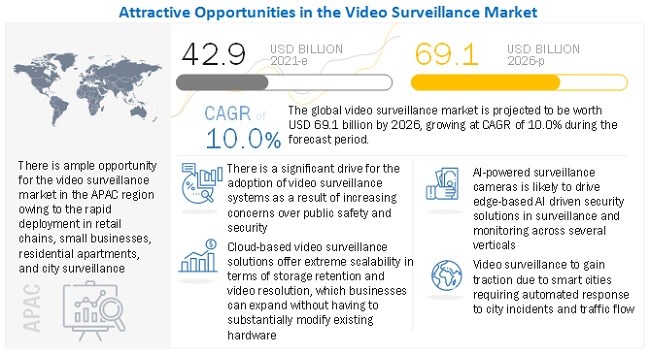
\includegraphics[width=12cm]{img/capitulo_2/surveillance-market.jpg}
        \caption{Proyección del mercado de la video-vigilancia.\\}
        Fuente: \cite{marketsandmarkets:market-surveillance}
        \label{fig:surveillance-market}
    \end{center}
    % \caption{Proyección del mercado de la video-vigilancia\\}    
\end{figure}

El aspecto más relevante del crecimiento en las oportunidades de este campo, se da en la implementación de nuevas características en este tipo de sistemas; gracias a las técnicas de visión por computadora e inteligencia artificial (I.A.), a la escalabilidad gracias al uso de servicios basados en la nube. Las ramas afines a la inteligencia artificial, como el Machine Learning (Aprendizaje Automático) y el Deep Learning (Aprendizaje profundo) han permitido lograr grandes avances en el campo de la video-vigilancia.\\

Para la implementación del prototipo propuesto, es necesario describir el marco teórico relevante en la captura de fotogramas de video, transmisión de datos por medio de la red por el protocolo tcp/ip, reconstrucción de información, consolidación y procesamiento de imágenes, como también la transmisión de video en vivo. A continuación se detallan los conceptos teóricos relevantes anteriormente descritos.\\

\section{Arquitectura de red}
Una arquitectura de red es un esquema completo de comunicación entre computadoras, el cual provee: un esquema de trabajo, un diseño principal, la construcción y manejo de una red. \cite[1]{networkProtocolos:handbook}. La arquitectura de red más importante es la de Interconexión de Sistemas Abiertos (OSI), desarrollada por la Organización Internacional para la Estandarización (ISO).\\

La arquitectura OSI, es un estándar abierto para la comunicación en red a través de diferentes equipos y aplicaciones. Aunque no está ampliamente implementado, el modelo de 7 capas OSI es considerado el modelo de arquitectura de red principal para la intercomputación y comunicación entre redes. En la figura \ref{fig:osi} se puede apreciar el modelo OSI de 7 capas, detallando a continuación las siguientes capas:

\begin{enumerate}
    \item Capa física (Physical)
    \item Capa de enlace (Data Link)
    \item Capa de red (Network)
    \item Capa de transporte (Transport)
    \item Capa de sesión (Session)
    \item Capa de presentación (Presentation)
    \item Capa de aplicación (Aplication)
\end{enumerate}

Este modelo se organiza de la siguiente manera: las capas 7 a 4 se ocupan de las comunicaciones de extremo a extremo entre la fuente de datos y destinos, mientras que las capas 3 a 1 se ocupan de las comunicaciones entre los dispositivos de red. Por otro lado, las siete capas del modelo OSI pueden dividirse en dos grupos: \textbf{capas superiores} (capas 7, 6 y 5) y \textbf{capas inferiores} (capas 4, 3, 2, 1).\\

\begin{figure}[H]
    \begin{center}
        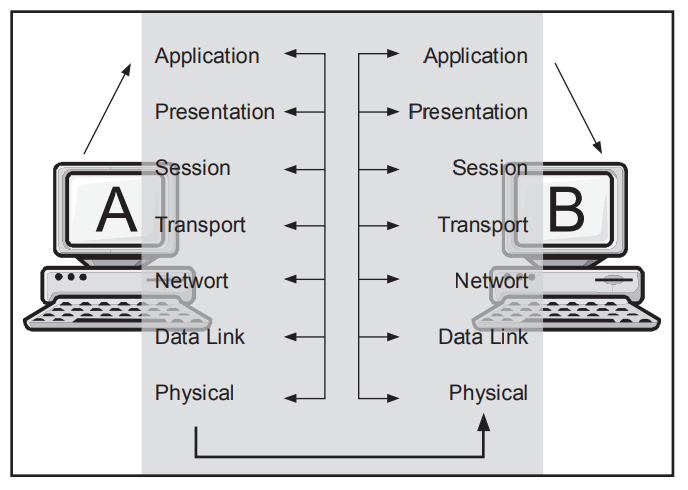
\includegraphics[width=9cm]{img/capitulo_2/capas.png}
        \caption{Esquema de capas del modelo OSI.\\}
        Fuente: \protect\cite[3]{networkProtocolos:handbook}
        \label{fig:osi}
    \end{center}
\end{figure}

Su contraparte en las arquitecturas de red del modelo OSI, es el modelo TCP/IP, que no sigue exactamente el modelo OSI. Desafortunadamente, no existe un acuerdo universal sobre cómo describir TCP/IP con un modelo en capas. Generalmente se acepta que TCP/IP tiene menos niveles (de tres a cinco capas) que las siete capas del modelo OSI. En la figura \ref{fig:tcpip} se visualiza las capas que se adoptan en esta arquitectura. 

\begin{figure}[H]
    \centering
    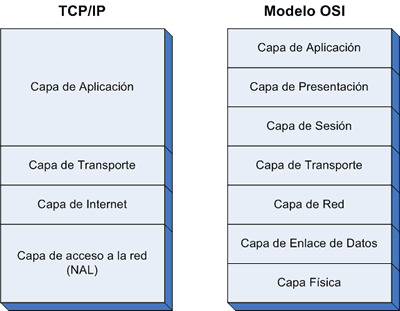
\includegraphics[width=8cm]{img/capitulo_2/tcp_ip_osi.jpg}\\
    \medskip
    \caption{Modelo TCP/IP frente al modelo OSI.\\}
    Fuente: \cite{tcpiposi}
    \label{fig:tcpip}
    % \end{center}
\end{figure}

La arquitectura TCP/IP omite algunas características que se encuentran en el modelo OSI, combina las características de algunas capas OSI adyacentes y separa otras. La estructura de 4 capas de TCP/IP (capa de aplicación, transporte, internet y acceso a la red) se construye a medida que la información se transmite de la capa de aplicacion a la capa de red física.\\

Cuando los datos son envíados, cada capa trata la información que recibe de la capa superior como datos y agrega información de control (encabezado) al frente de esos datos y luego los pasa a la capa inferior. Cuando se reciben los datos, se lleva a cabo el procedimiento opuesto ya que cada capa procesa y elimina su encabezado antes de pasar los datos a la capa superior.\\

\subsection{Protocolos}
El modelo OSI, y cualquier otro modelo de comunicación de red, proporciona solo un esquema conceptual para la comunicación entre computadoras, pero el modelo en sí mismo no proporciona métodos específicos de comunicación \cite{wikipedia:modeloosi}. La comunicación real está definida por varios protocolos de comunicación.\\

En el contexto de la comunicación de datos, un protocolo es un conjunto formal de reglas, convenciones y estructuras de datos que determinan cómo las computadoras y otros dispositivos de red intercambian información a través de una red. Este método estándar permite la comunicación entre procesos (que potencialmente se ejecutan en diferentes equipos) y agrega un conjunto de reglas y procedimientos que deben respetarse para el envío y la recepción de datos a través de una red.\\

Similar a la manera de hablar el mismo lenguaje entre dos personas; un protocolo, simplifica la comunicación entre dispositivos. La arquitectura de red proporciona solo un esquema conceptual para la comunicación. El modelo no proporciona métodos específicos de comunicación, sino mas bién, la comunicación real está definida por varios protocolos de comunicación que son usados en la comunicación analógica y digital, y pueden ser usados en el procesos de transferencia de archivos y acceso a internet.\\

Los protocolos de comunicación en red más populares, incluyen:

\begin{itemize}
    \item \textbf{Automatización}: Automatizan diferentes procesos tanto en entornos comerciales como personales: en edificios inteligentes, tecnología en la nube o vehículos autónomos.
    \item \textbf{Mensajeria Instantánea}: La comunicación basada en texto, en teléfonos inteligentes y computadoras suceden debido a una serie de diferentes protocolos de mensajeria instantánea.
    \item \textbf{Enrutamiento}: Protocolos de enrutamiento permiten la comunicación entre routers y otros dispositivos de red.
    \item \textbf{Transferencia de archivos}: Envio de archivos por medio de un canal de comunicación.
    \item \textbf{Acceso a Internet}: El protocolo de Internet (IP) permite que los datos sean enviados entre dispositivos por medio de la red de internet.
\end{itemize}

A continuación se detallan algunos de los protocolos más conocidos:
\begin{itemize}
    \item \textbf{HTTP - Protocolo de transferencia de hipertexto}: Este protocolo de internet define la manera en la que los datos son enviados por internet y determina como los navegadores web y buscadores deben responder a determinados comandos.
    \item \textbf{SSH - Secure Socket Shell}: Este protocolo provee un acceso seguro al dispositivo, incluso si se encuentra en una red no segura. SSH es particularmente usado por administradores de red quienes manejan diferentes sistemas de manera remota.
    \item \textbf{SMS - Servicio de envío de mensajes cortos}: Este protocolo ha sido creado para enviar y recibir mensajes de texto sobre redes de telefonía celular. SMS refiere exclusivamente a mensajes basados en texto. Las imágenes, videos u otro contenido multimedia requiere el protocolo de Servicio de mensajeria multimedia (MMS), que es una extensión del protocolo SMS.
    \item \textbf{ICMP - Protocolo de control de mensajes de Internet}: Trabaja como asistente del protocolo de Internet y se encarga de identificar fallos en la información y enviar mensajes de error hacia el usuario o servidor. Por ejemplo, si una dirección de este no está disponible o si una solicitud presenta fallas.
    \item \textbf{SMTP - Protocolo de transferencia de correo simple}: Este se encarga del intercambio de datos por texto en mensajes de correo electrónico entre ordenadores por medio de la red.
\end{itemize}

\subsection{Modelo cliente-servidor}
El modelo cliente-servidor es una estructura de aplicación distribuida que divide tareas o cargas de trabajo entre los proveedores de un recurso o servicio, denominados servidores, y los solicitantes del servicio, denominados clientes \cite{wikipedia:cliente_servidor}. A menudo, los clientes y los servidores se comunican a través de una red informática en hardware independiente, pero tanto el cliente como el servidor pueden residir en el mismo sistema.\\

Un servidor ejecuta uno o más programas de servidor, que comparten sus recursos con los clientes. Un cliente normalmente no comparte ninguno de sus recursos, pero solicita contenido o servicio de un servidor. En la figura \ref{fig:client_server} se aprecia un diagrama que representa el modelo cliente-servidor, donde los clientes acceden al servicio del servidor por medio de la misma red de internet.\\

\begin{figure}[H]
    \begin{center}
        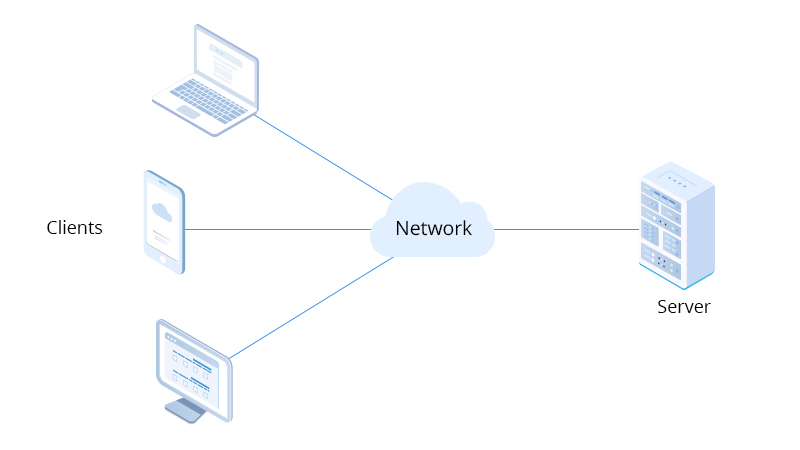
\includegraphics[width=10cm]{img/capitulo_2/client-server.jpeg}
        \caption{Ilustración del Modelo cliente-servidor\\}
        Fuente: \cite{clientserver}
        \label{fig:client_server}
    \end{center}
\end{figure}

Por lo tanto los clientes, inician sesiones de comunicación con los servidores, que esperan las solicitudes entrantes. Para mencionar algunos ejemplos de aplicaciones informáticas que utilizan este modelo cliente-servidor son el correo electrónico, la impresión en red y la World Wide Web (Internet).\\

La comunicación entre el cliente y el servidor se realiza por medio de una conexión o enchufe ``socket'' el cual define la dirección y puerto por la cual va a ser enviada y/o recibida la información entre ambos actores. En la figura \ref{fig:socket_request} se visualiza la forma en la que se realiza la conexión entre el lado del cliente y el servidor por medio de un conector o ``socket''. En el lado del cliente: este conoce el nombre de host de la máquina en la que se ejecuta el servidor y el número de puerto en el que escucha el servidor.\\

Para realizar una solicitud de conexión, el cliente intenta conectarse con el servidor en la máquina y el puerto del servidor, además el cliente también necesita identificarse ante el servidor, para vincularse a un número de puerto local que se utiliza durante esa conexión. Normalmente lo asigna el sistema.\\

\begin{figure}[H]
    \begin{center}
        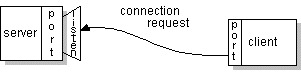
\includegraphics[width=6cm]{img/capitulo_2/socket_request.jpg}
        \caption{Solicitud de conexión por medio de un socket\\}
        Fuente: \cite{socketconnection}
        \label{fig:socket_request}
    \end{center}
\end{figure}

Si la solicitud tiene éxito, el servidor acepta la conexión. Después esta aceptación, el servidor obtiene un nuevo ``socket'' o conector vinculado al mismo puerto local como también tiene su punto final remoto establecido en la dirección y el puerto del cliente. En la figura \ref{fig:socket_connection} se visualiza el comportamiento del conector después de la aceptación a la petición de conexión del cliente; una vez establecida la conexión, el servidor necesita un nuevo socket para continuar escuchando las futuras solicitudes de conexión mientras atiende las necesidades del cliente conectado.\\

\begin{figure}[H]
    \begin{center}
        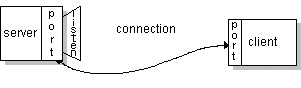
\includegraphics[width=6cm]{img/capitulo_2/socket_connection.jpg}
        \caption{Conexión establecida entre sockets\\}
        Fuente: \cite{socketconnection}
        \label{fig:socket_connection}
    \end{center}
\end{figure}

% El protocolo de Control de Transmisión (TCP) es uno de los protocolos fundamentales de internet. Fue creado entre los años 1973-1974 por Vint Cerf y Robert Kahn. Este es uno de los principales protocolos de la ``capa de transporte'' del modelo TCP/IP.<cita> A nivel de aplicación, posibilita la administración de datos que vienen del nivel más bajo del modelo, o van hacia él, (es decir, al protocolo IP). Cuando se proporcionan los datos al protocolo IP, este los agrupa en datagramas IP, fijando el campo del protocolo en 6 (para que sepa con anticipación que el protocolo es TCP). \\

% El protocolo TCP verifica los datos que son enviados por Internet, mientras que el segundo, IP o Internet protocol, se encarga de enviar esos datos a su destino suministrándoles un encabezado para identificarlos. Tanto uno como el otro son protocolos diferentes, que incluso habitan en capas diferentes del modelo OSI, pero son tan importantes el uno para el otro, que suele llamárseles TCP/IP como si fueran uno solo porque trabajan en conjunto y se necesitan. TCP e IP son la base de todo el Internet que conocemos actualmente.\\

% Las principales características del protocolo TCP son las siguientes: 

% \begin{itemize}
%     \item Ofrece soporte a la mayoria de las aplicaciones más populares de internet, incluidas HTTP, SMTP, SSH y FTP. 
%     \item Organiza los datagramas nuevamente en orden cuando vienen del protocolo IP.
% \end{itemize}

El flujo general de interacción es como sigue: el servidor TCP establece un conector en una determinada dirección y puerto, y se mantiene escuchando constantemente si algún conector cliente (que conoce la dirección y puerto del servidor) solicita una conexión; cuando el servidor acepta la conexión, se brinda un nuevo puerto diferente de manera automática para comunicarse exclusivamente con la nueva coexión y mantiene el puerto original a la escucha de nuevas conexiones, como se ve en la figura \ref{fig:tcp_flow}. Cuando se establece esta conexión, tanto como el cliente y el servidor pueden enviar y recibir datos. Cuando el cliente decide cerrar la conexión, el servidor pone de nuevo el puerto utilizado anteriormente como disponible.\\

\begin{figure}[H]
    \begin{center}
        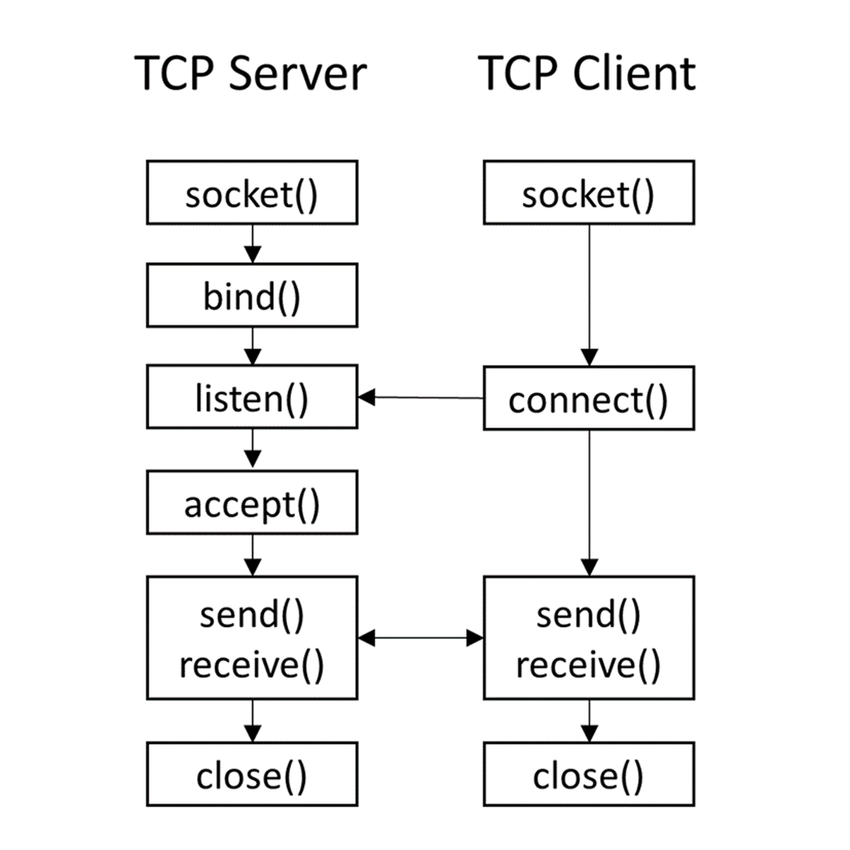
\includegraphics[width=6.4cm]{img/capitulo_2/tcp.png}
        \caption{Flujo de interacción entre servidor y cliente TCP.\\}
        Fuente: \cite{tcpsocket}
        \label{fig:tcp_flow}
    \end{center}
\end{figure}

A continuación se detalla los métodos que se muestran en la figura \ref{fig:tcp_flow}:
\begin{itemize}
    \item socket(): Crea un punto final para la comunicación en el servidor.
    \item bind(): Asigna un número único al socket y reservar una combinación única de dirección IP y puerto para el socket creado.
    \item listen(): Espera a que un cliente se conecte.
    \item accept(): Recibe una solicitud de conexión de un socket de cliente.
    \item connect(): El cliente y el servidor están conectados entre sí.
    \item send()/recieve(): Intercambian datos entre el cliente y el servidor
    \item close(): El servidor y el cliente cortan la conexión.
\end{itemize}

% En el lado del cliente: el cliente conoce el nombre de host de la máquina en la que se ejecuta el servidor y el número de puerto en el que escucha el servidor. Para realizar una solicitud de conexión, el cliente intenta reunirse con el servidor en la máquina y el puerto del servidor. El cliente también necesita identificarse ante el servidor para vincularse a un número de puerto local que utilizará durante esta conexión. Normalmente lo asigna el sistema.

% En el lado del cliente, si se acepta la conexión, se crea correctamente un socket y el cliente puede usar el socket para comunicarse con el servidor. El cliente y el servidor ahora pueden comunicarse escribiendo o leyendo desde sus sockets.

% Un punto final es una combinación de una dirección IP y un número de puerto. Cada conexión TCP se puede identificar de forma única por sus dos puntos finales. De esa manera, puede tener múltiples conexiones entre su host y el servidor.

Los clientes y servidores intercambian mensajes en un patrón de mensajería de solicitud-respuesta. Para comunicarse, las computadoras deben tener un lenguaje común y deben seguir reglas para que tanto el cliente como el servidor sepan qué esperar. El idioma y las reglas de comunicación se definen en un protocolo de comunicaciones. Todos los protocolos operan en la capa de aplicación.\\

% El protocolo de la capa de aplicación define los patrones básicos del diálogo. Para formalizar aún más el intercambio de datos, el servidor puede implementar una interfaz de programación de aplicaciones (API).[3] La API es una capa de abstracción para acceder a un servicio. Al restringir la comunicación a un formato de contenido específico, facilita el análisis. Al abstraer el acceso, facilita el intercambio de datos entre plataformas.[4]
\subsection{HTTP}
El protocolo de transferencia de hipertexto (HTTP) es el más utilizado en Internet. Se usa en cada transacción de la Web (www) y permite la transferencia de archivos (principalmente, en formato HTML) entre un navegador (cliente) y un servidor web. HTTP define la sintaxis y la semántica que utilizan los elementos software de la arquitectura web (clientes, servidores, proxies) para comunicarse. Este protocolo se orienta a las transacciones y sigue el esquema ``Petición - Respuesta'' entre un cliente y un servidor. En la figura \ref{fig:http} se aprecia la interacción entre el cliente y el servidor web.

\begin{figure}[H]
    \begin{center}
        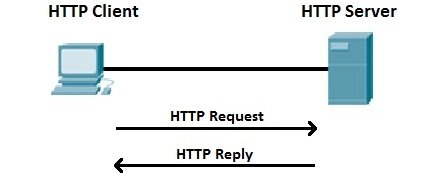
\includegraphics[width=8cm]{img/capitulo_2/http1.jpg}
        \caption{Interacción del protocolo HTTP.\\}
        Fuente: \cite{http}
        \label{fig:http}
    \end{center}
\end{figure}

Este protocolo se compone las siguientes características:
\begin{itemize}
    \item El cliente que efectúa la petición (un navegador o un spider) es denominado ``user agent'' (agente del usuario). 
    \item La información transmitida se denomina ``recurso'' y se identificada mediante una cadena de caracteres definida como dirección URL.
    \item Los recursos pueden ser archivos, el resultado de la ejecución de un programa, una consulta a una base de datos, la traducción automática de un documento, etc.
\end{itemize}

\section{Inteligencia Artificial}
La Inteligencia Artificial (I.A.), como área de estudio de las ciencias de la computación, en los últimos tiempos dejó de estar reservada para la investigación y pasó a formar parte del desarrollo de la sociedad. El cerebro es el órgano más increible del cuerpo humano; establece la forma en la que percibimos las imágenes, sonido, olores, sabores y el tacto; por lo tanto permite al ser humano almacenar recuerdos, experimentar emociones e incluso soñar. Sin él, el ser humano sería un organismo primitivo, incapaz de otra cosa que el más simple de los reflejos. Por lo tanto, el cerebro es lo que hace inteligente al ser humano \cite{intro_ia}.\\

Durante décadas se ha investigado para construir máquinas inteligentes con cerebros como el del ser humano; asistentes robotizados para limpiar los hogares, coches que se conducen por solos, microscopios que detecten enfermedades automáticamente. Pero en la construcción de estas máquinas artificialmente inteligentes se presentan problemas computacionales complejos; problemas que el cerebro humano puede resolver en una fracción de segundos. Las formas de analizar y resolver este tipo de problemas, son estudiados por la inteligencia artificial.

\begin{figure}[H]
    \begin{center}
        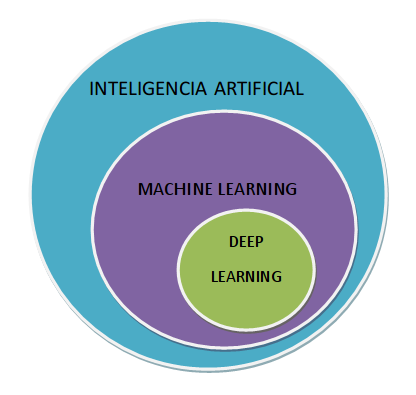
\includegraphics[width=6cm]{img/capitulo_2/ia.png}
        \caption{La Inteligencia Artificial y sus sub-areas\\}
        Fuente: \cite{ia}
        \label{fig:ia}
    \end{center}
\end{figure}

A menudo los conceptos de Inteligencia Artificial, Aprendizaje Automático (Machine Learning) y Aprendiazaje Profundo (Deep Learning) son usados de manera indistinta. Por los años `80 la Inteligencia Artificial era una característica que se alcanzaba al definir un conjunto de reglas que decían que hacer en un determinado momento, de esta manera un sistema `inteligente' solo obedecía reglas de acción programadas \cite{researchgate:ia}. En la figura \ref{fig:ia} se ilustra como la Inteligencia Artificial engloba los subcampos de estudio como son el Machine Learning y el Deep Learning.

\subsection{Redes Neuronales}
Las redes neuronales artificiales, son un modelo inspirado en el funcionamiento del cerebro humano. Está formado por un conjunto de nodos conocidos como neuronas artificiales que están conectadas y transmiten señales entre sí. Estas señales se transmiten desde la entrada hasta generar una salida. En la figura \ref{fig:classical_ml} se aprecia la estructura propia de una neurona artificial.\\

\begin{figure}[H]
    \begin{center}
        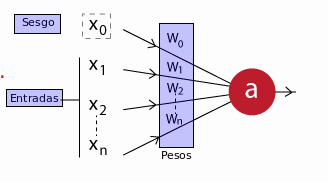
\includegraphics[width=6cm]{img/capitulo_2/neurona.png}
        \caption{Ilustración de una Neurona artificial\\}
        Fuente: \cite{tensorflow_neurona}
    \label{fig:classical_ml}
    \end{center}
\end{figure}

El objetivo principal de un modelo neuronal, es aprender por medio de la modificación automática de si misma, llegando a realizar tareas complejas que no podrían ser realizadas mediante programación clásica basada en reglas. De esta forma se pueden automatizar funciones que al principio solo podrían ser realizadas por personas. Semejante al del cerebro humano, las redes neuronales reciben una serie de valores de entrada, donde cada una de estas llegan a un nodo llamado neurona.\\

Las neuronas de una red están a su vez agrupadas en capas formando una red neuronal. Cada una de las neuronas de la red poseen un peso, que es un valor numérico con el que modifica la entrada recibida. Los nuevos valores obtenidos por las neuronas continúan su camino por la red. En la figura \ref{fig:estructura_red_neuronal} se aprecia el funcionamiento anteriormente descrito.\\

\begin{figure}[H]
    \begin{center}
        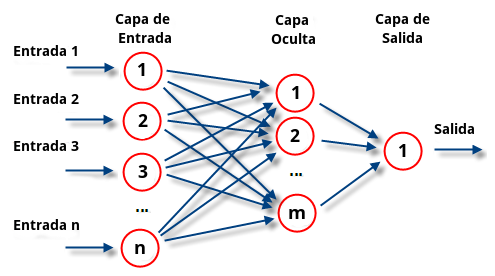
\includegraphics[width=6cm]{img/capitulo_2/Redes_neuronales_esquema.png}
        \caption{Modelo de capas de una red neuronal.\\}
        Fuente: \cite{perceptron_multicapa}
        \label{fig:estructura_red_neuronal}
    \end{center}
\end{figure}

Cuando este proceso llega al final de la red, se obtiene una salida que será la predicción calculada por la red. Cuantas más capas posea la red y aumente la complejidad de sus conexiones; mas complejas serán las funciones que pueda realizar. Para que una red neuronal realice las funciones deseadas, es necesario la ejecución del entrenamiento correspondiente.\\

El entrenamiento de la red neuronal se realiza por medio de la modificación de los pesos de sus neuronas para que consiga extraer los resultados deseados. Para ello, se introduce datos de entrenamiento en la red, según el resultado obtenido y el error se modifican los pesos de las neuronas en función de cuanto haya contribuido cada neurona a dicho resultado. Este método es conocido como ``backpropagation'' o propagación hacia atrás. Con este método se consigue que la red ``aprenda'', consiguiendo un modelo capaz de obtener resultados muy acertados incluso con datos muy diferentes a los de su entrenamiento \cite{atriainnovation:ia}.\\

Estas redes neuronales son utilizadas para tareas de predicción y clasificación. Esta técnica se ha convertido en una pieza clave para el desarrollo de la Inteligencia Artificial. Como se describió previamente, es uno de los principales campos de investigación y el que más ha evolucionado con el tiempo, ofreciendo cada vez soluciones más complejas y eficientes.\\

\subsubsection{Redes neuronales convolucionales}
Dentro del conjunto de tipos de redes neuronales están las convolucionales, que se usan en el campo de la visión artificial. Las redes neuronales convolucionales representan un algoritmo de Aprendizaje Profundo (Deep Learning) que está diseñado para trabajar con imágenes. Toma las imágenes como entrada, les asigna un valor (peso) a ciertos elementos en la imagen para su clasificación.\\

\begin{figure}[H]
    \begin{center}
        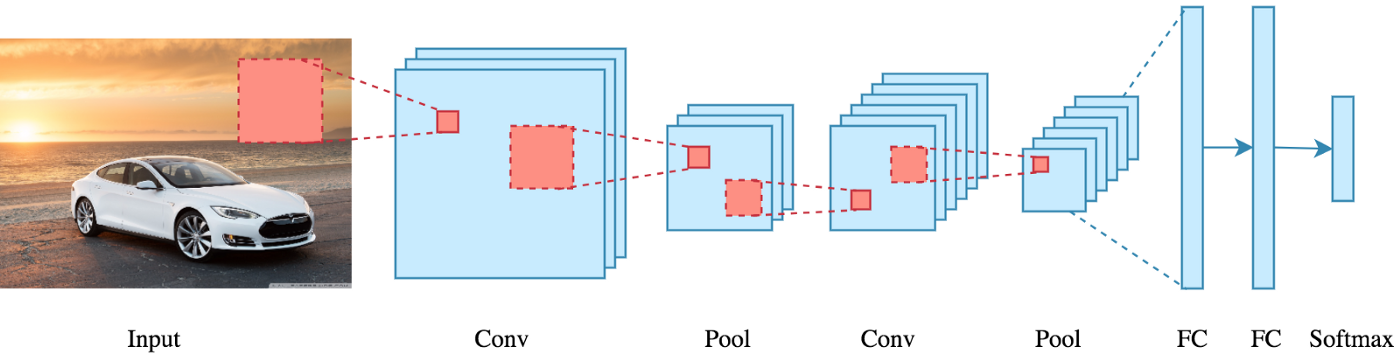
\includegraphics[width=11cm]{img/capitulo_2/convolucional.png}
        \caption{Ilustración de una Red Neuronal Convolucional.\\}
        Fuente: \cite{intro_redes_neuronales}
        \label{fig:red_neuronal_convolucional}
    \end{center}
\end{figure}

Estas redes han contribuido en el desarrollo y perfeccionamiento del campo de la visión por computadora. Las redes convolucionales contienen varias capas ocultas como se ilustra en la figura \ref{fig:estructura_red_neuronal}, donde las primeras puedan detectan líneas, curvas y así se van especializando hasta poder reconocer formas complejas como un rostro, siluetas, etc. \cite{convolutional:ia}. \\

\begin{figure}[H]
    \begin{center}
        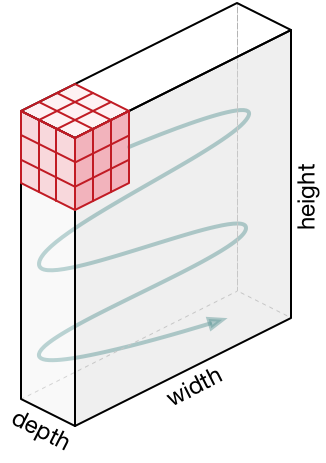
\includegraphics[width=2cm]{img/capitulo_2/kernel.png}
        \caption{Movimiento del Kernel.\\}
        Fuente: \cite{comprension_redes_neuronales}
        \label{fig:kernel}
    \end{center}
\end{figure}

Estas redes funiconan en base de convoluciones. Este proceso consiste en tomar un grupo de píxeles de la imagen de entrada e ir realizando un producto escalar con un kernel. El kernel recorrerá todas las neuronas de entrada y obtendremos una nueva matriz, la cual será una de las capas ocultas. En el caso de que la imagen sea de color se tendrán 3 kernels del mismo tamaño que se sumarán para obtener una imagen de salida. El ``kernel'' dentro las redes convolucionales es considerado como un filtro que se aplica para extraer ciertas características importantes o patrones. Se usa para detectar bordes, enfoque, desenfoques, y características de la imagen por la convolución entre la imagen y el kernel. Este proceso se desarrolla entre la imagen y el kernel, con la finalidad de que el kernel recorra toda la imagen (pixel por pixel). Por lo general, el kernel es de menor tamaño que la imagen permitiendo multiplicar el kernel con la porción de imagen escogida, realiza un producto escalar a medida que el kernel se va desplazando; por esta razón es un proceso iterativo. Las tareas comunes de este tipo de redes son: detección o categorización de objetos, clasificación de escenas y clasificación de imágenes en general.\\

% Tiene dos usos:
% El primero es para que al realizar la convolución la imagen resultante sea de igual tamaño que la imagen original.
% El segundo es cuando se tiene información relevante en las esquinas de la imagen por lo que al realizar convolución el filtro pasa más por el centro de la imagen que en las esquinas, por lo que se aplica el padding para tener la información más relevante cerca del centro.\\

\section{Machine Learning (Aprendizaje de Máquina)}
Es un subcampo de la Inteligencia Artificial cuyo objetivo es entender la estructura de la información y ajustar estos datos en modelos que puedan ser entendidos y utilizados por las personas. \cite{digitalocean:machinelearning}. A diferencia de la computación tradicional, donde los algoritmos resuelven problemas específicos, los algoritmos de Machine Learning entrenan a las computadoras con datos de entrada y emplean análisis estadístico para generar valores de salida que se clasifican según a un rango específico. Por eso el Machine Learning facilita a las computadoras construir modelos a partir de datos ejemplo para automatizar el proceso de toma de decisiones basados en estos datos.\\

\begin{figure}[H]
    \begin{center}
        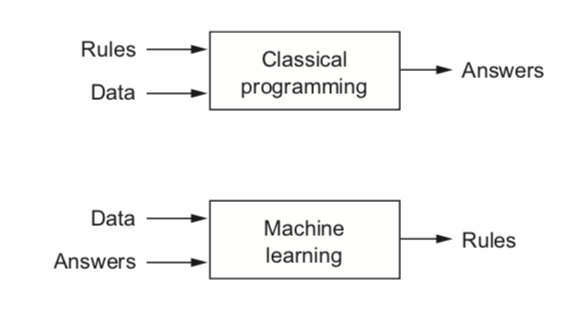
\includegraphics[width=9cm]{img/capitulo_2/machinelearning.png}
        \caption{Diferencias entre programación clásica y M.L.\\}Fuente: \cite{classicprog_and_ml}
        \label{fig:classical_ml}
    \end{center}
\end{figure}

En la figura \ref{fig:classical_ml} se visualiza la diferencia y similitud entre la programación clásica de la inteligencia artificial de los años `80 y las novedosas técnicas del aprendizaje automático. La programación clásica necesita de reglas y datos de entrada para que esta funcione como un sistema inteligente y pueda dar una respuesta, mientras que el Machine Learning necesita de datos y sus respectivas respuestas esperadas, para identificar patrones que los relacionen y asi desarrollar reglas que generan respuestas para nuevos datos.

\subsection{Métodos de Machine Learning}
En el Machine Learning, las tareas se clasifican en grandes categorias, las cuales estan basadas en el modo en el que el ``aprendizaje'' es ejecutado. Los métodos más adoptados en el Machine Learning son: el aprendizaje supervisado y el no supervisado.\\

% que entrena un algoritmo basado en un ejemplo de entrada y salida el cual esta categorizado por un humano, y el aprendizaje no supervisado, que proporciona el algoritmo sin ningún dato categorizado permitiendo encontrar una estructura dentro de los datos de entrada.\

\subsubsection{Aprendizaje Supervisado}
La computadora es provista de entradas ejemplo las cuales se categorizan con sus respectivas salidas esperadas. El propósito de este metodo consiste en que el algoritmo pueda  ``aprender'' comparando la actual salida con las salidas esperadas para encontrar errores y en consecuencia modificar el modelo. El aprendizaje supervisado por lo tanto usa patrones para predecir valores categorizados en datos no categorizados.\\

\subsubsection{Aprendizaje No Supervisado}
La información provista a la computadora no está categorizada, por lo que los algoritmos de aprendizaje buscan similitudes entre los datos de entrada. Como los datos no etiquetados son más abundantes que los datos etiquetados, los métodos de aprendizaje automático que facilitan el ``aprendizaje'' pasan a ser más importantes.\\

\section{Deep Learning (Aprendizaje profundo)}
En la figura \ref{fig:ia}, se visualiza que el aprendizaje profundo es un subcampo dentro del Machine Learning, el cual hace uso de distintas redes neuronales para lograr el ``aprendizaje'' de sucesivas capas de representación que son relevantes para los datos. El término Deep ``profundo'', hace referencia a la cantidad de capas de representación que se utilizan en un modelo; en general es posible utilizar decenas incluso cientos capas de representación, los cuales aprenden de forma automática a medida que el modelo es entrenado con los datos \cite{iaarbook:artificialvision}.

\section{Técnicas de visión por computadora}
La visión por computadora es una técnica de recolección de información que surge por la inspiración en el sistema visual humano, el cual es la principal fuente de información para el cerebro. Su meta es de modelar y automatizar el proceso de reconocimiento visual de objetos en la vida real.\\

De los cinco sentidos que poseen las personas, la vista es la más importante. Por lo tanto la visión, es una tarea de procesamiento de información; pero tiene un grado de complejidad elevado, saber que es lo qué hay en el mundo, el cerebo humano deben se capaz de representar esta información sobre el color, la forma, movimiento, detalle y belleza de los objetos. \cite{iaarbook:artificialvision}\\

La visión por computadora o visión artificial compone de un conjunto de herramientas y métodos que permiten obtener, procesar y analizar imágenes del mundo real por medio de una computadora. Estos métodos van a permitir automatizar un amplio conjunto de tareas al aportar a las computadoras información que es necesaria para la toma de desiciones en sus tareas asignadas. Esta técnica trata de imitar a la visión humana, usando geometría y un enfoque estadístico para solucionar el problema.\\

\subsection{Aplicaciones}
Esta rama de la Inteligencia Artificial aún sigue en investigación y mejoras donde sus aplicaciones más comunes son:

\begin{itemize}
    \item \textbf{Reconocimiento óptico de caracteres:} Detección automática de símbolos que pertenecen a un alfabeto.
    \item \textbf{Inspección robotizada:} Revisión rápida de piezas para garantizar la calidad de componentes fabricados.
    \item \textbf{Modelado 3D:} Construcción de modelos 3D a partir de fotografías.
    \item \textbf{Imágenes médicas:} Análisis de radiografías.
    \item \textbf{Conducción segura:} Detección de obstáculos por medio de un sistema de conducción asistida por cámaras.
    \item \textbf{Vigilancia:} Monitoreo de intrusos, análisis del tráfico vial, monitoreo de piscinas, etc.
    \item \textbf{Detección de rostros:} Mediante algoritmos de reconocimiento facial se reconocen rostros usados en métodos de biometría.
\end{itemize}

\subsection{Librerias}
Una de las librerias mas utilizadas para las técnicas de vision por computadora es OpenCV. Es una biblioteca de uso libre para el desarrollo de aplicaciones usando visión artificial desarrollada por Intel. Esta libreria reune diversas caracteristicas que la hacen popular, por ejemplo: 
\begin{itemize}
    \item Permite su uso para fines comerciales y de investigación.
    \item Se encuentra disponible par varias plataformas como ser GNU/Linux, Mac OS, Windows y Android.
    \item Documentación completa y explicada, con una comunidad de desarrolladores activa.
    \item El procesamiento de imágenes en su escalado, eliminación de ruido y formateo de imagen y video.
    \item El uso y modificación de sus 2500 modelos pre-optimizados que son incluidos en la libreria, acorde a las necesidades del usuario.
    \item El uso del estado del arte de modelos de visión por computadora como también de aprendizaje de máquina (Machine Learning).
    \item El desarrollo de modelos en varias categorías de investigación como ser: reconocimiento facial, detección y seguimiento de objetos, extracción de modelos 3D, etc.
\end{itemize}

\begin{figure}[H]
    \begin{center}
        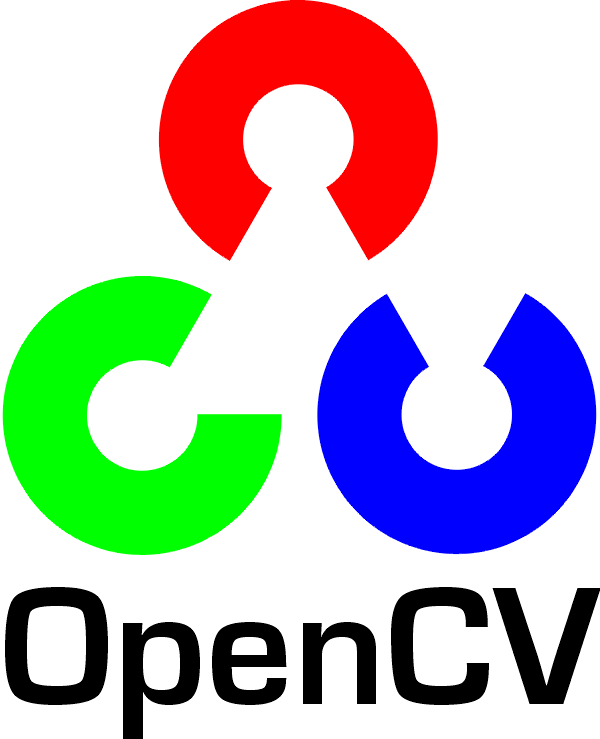
\includegraphics[width=2cm]{img/capitulo_2/cv2_logo.png}
    \end{center}
    \caption{Logotipo de la libreria\\Fuente: Web}
    \label{fig:cv2_logo}
\end{figure}

% Una de las características mas interesantes de OpenCV es el reconocimiento facial. OpenCV, en su extensa biblioteca de funciones, brinda las capacidades para realizar las tareas de preprocesamiento sin ningún problema, así como los algoritmos de predicción. Además de usar el algoritmo de detección de objetos, es posible usar el seguimiento de objetos, para identificar rostros en una transmisión de video. OpenCV incluso posee funciones para configurar fácilmente el modelo en una transmisión en vivo, como en un video pregrabado \cite{medium:opencv}. 

Existen otras librerias que no son tan populares y representan un pago adicional.

\section{Streamming}
Este término también se denomina como transmisión, lectura en continuo, difusión en flujo, lectura en tránsito, difusión en continuo, descarga continua. Es la distribución digital de multimedia a través de una red de computadoras, de manera que el usuario consume el producto (generalmente archivo de vídeo o audio) en paralelo mientras se descarga \cite{streamming:austerberry}.\\

Se aplica habitualmente a la difusión de audio o vídeo. El streaming requiere una conexión por lo menos de igual ancho de banda que la tasa de transmisión del servicio. El streaming de vídeo se popularizó a fines de la década de 2000, cuando el ancho de banda se hizo lo suficientemente barato para gran parte de la población. Sin embargo, con la tecnología del streaming, un archivo puede descargarse y reproducirse al mismo tiempo, con lo que el tiempo de espera es mínimo \cite{streamming:austerberry}. El streamming permite la reproducción directa del contenido multimedia, sin la necesidad de almacenar en memoria la información para después reproducirla, como se puede ver en la figura \ref{fig:stream}.\\

\begin{figure}[H]
    \begin{center}
        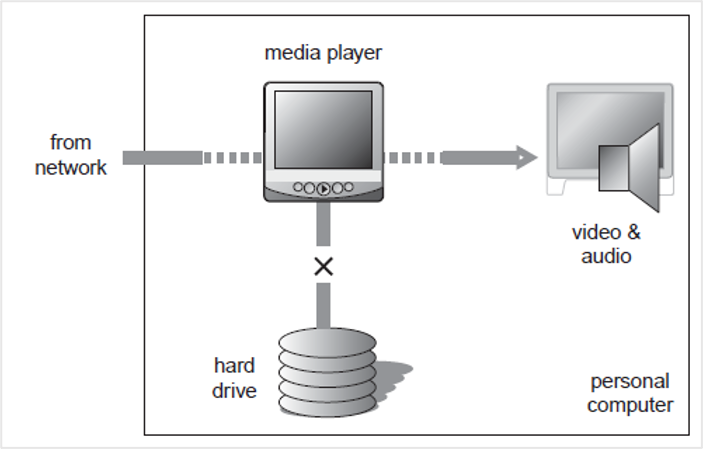
\includegraphics[width=8cm]{img/capitulo_2/stream.png}
        \caption{Streaming en un servidor web.\\}
        Fuente: \cite{streamming:austerberry}
        \label{fig:stream}
    \end{center}
\end{figure}

El servidor más utilizado para la transmisión de contenidos multimedia es el servidor web, tipificado por Apache. Los servidores Web utilizan HTTP a través de TCP/IP para entregar sus páginas HTML y archivos de imagen asociados. El protocolo TCP/IP se utiliza como la capa de transporte a través de Internet. Los archivos se descargan a la memoria caché del navegador web más rápido de lo que el sistema permite. TCP incorpora control de flujo para gestionar la velocidad de descarga.\\
\subsection{Servidor web para el Streaming de contenido multimedia}

El servidor web reproduce contenido multimedia de la siguiente forma: el servidor mediante una aplicación proporciona una dirección que permite acceder a un archivo multimedia por medio de un reproductor. Luego que se establece una conexión al servidor web mediante el mismo enlace, se manda una señal para que el servidor transmita el contenido. El servidor web redirige al reproductor a un servidor streaming para luego recién realizar la reproducción del contenido digital, como se observa en la figura \ref{fig:streamming}.\\

Un servidor web no realiza este proceso sin un servidor Streaming de por medio; permite la descarga del archivo en su totalidad para que después se realice la reproducción por parte del reproductor. El servidor streaming decodifica el bitrate en el que se codificó. Los oyentes deben tener instalado un reproductor multimedia en su ordenador, pero también se puede escuchar la emisión sin necesidad de éste último. Se podría utilizar: Windows Media Player, VLC, o algún software compatible.\\

\begin{figure}[H]
    \begin{center}
        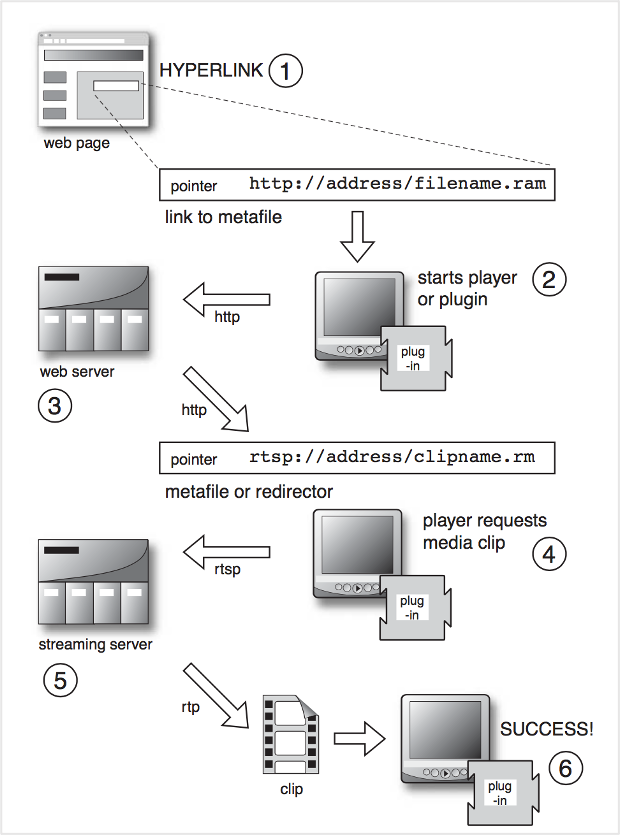
\includegraphics[width=12cm]{img/capitulo_2/streamming.png}
        \caption{Streaming en un servidor web.\\}
        Fuente: \cite{streamming:austerberry}
        \label{fig:streamming}
    \end{center}
\end{figure}

El termino bitrate se refiere a la calidad de la señal, usualmente se utilizan 24, 32, 48, 64 kbps pero si se requiere se puede emitir a un bitrate superior, por ejemplo 96 kbps o 128 kbps. Se debe tener en cuenta que a mayor bitrate es necesario mayor ancho de banda, así como mayor será el costo. Sin la tecnología de Streaming, para reproducir un archivo multimedia, seria necesario descargar en memoria del computador para después recién reproducirlo.\\

\subsubsection{Http Live Streaming (HLS)}
HLS es un protocolo utilizado para enviar audio y video sobre HTTP, soporta bitrate adaptivo y es compatible con la mayoría de los dispositivos. Este protocolo fue desarrollado por Apple y puede ser utilizado tanto para video en vivo como video en demanda. Entre sus características importantes se tiene:

\begin{itemize}
    \item Se adapta a las condiciones de la red. Según el ancho de banda de internet del espectador, entrega una calidad o bitrate adecuado.
    \item Puede ser entregado desde un servidor tradicional de HTTP.
    \item Es protegido con encriptado o autenticación con el fin de proteger derechos de autor.
\end{itemize}

El flujo del protocolo es como sigue: 
\begin{enumerate}
    \item El archivo de video se codifica con compresión de video H.264 y compresión de Audio AAC.
    \item Selecciona MPEG2-TS como contenedor de video, esto lo hace normalmente un encoder de video.
    \item Cuando es codificado el video, se realiza un proceso de segmentación.  Este proceso realiza cortes del video cada ciertos segundos, usualmente cada 10 segundos. A estos fragmentos se les conoce como segmentos o ``chunks'' de video.
    \item Se genera un archivo índice. Este archivo contiene la información de los segmentos y en donde se encuentran para que el player los descargue. Este mismo proceso se realiza tanto para video en vivo o video en demanda (video almacenado).
    \item Cuando se decide encriptar la información, se ejecuta un algoritmo para proteger cada uno de los segmentos. Donde el player que tenga la llave para desencriptarlos puede ver el contenido.
    \item  Estas llaves pueden ser estáticas o dinámicas. Puede generarse una llave para todos los videos o una llave por video.
\end{enumerate}
La URL de reproducción tiene la siguiente forma:
\begin{center}
    \verb|http://nombre-del-dominio/directorio-del-video/mi-video.m3u8|    
\end{center}

Usando el mismo protocolo que impulsa la web, HLS comparte contenido usando servidores web y redes de entrega de contenido ordinarios. HLS está diseñado para brindar confiabilidad y se adapta dinámicamente a las condiciones de la red al optimizar la reproducción para la velocidad disponible de las conexiones por cable e inalámbricas.\\

% Es un protcolo (HLS) envía audio y video a través de HTTP desde un servidor web común para su reproducción en dispositivos basados en iOS, incluidos iPhone, iPad, iPod touch y Apple TV, y en computadoras de escritorio (macOS). Usando el mismo protocolo que impulsa la web, HLS implementa contenido usando servidores web y redes de entrega de contenido ordinarios. HLS está diseñado para brindar confiabilidad y se adapta dinámicamente a las condiciones de la red al optimizar la reproducción para la velocidad disponible de las conexiones por cable e inalámbricas.
En la figura, \ref{fig:hls} se visualiza un esquema que representa el proceso de que sigue HLS. El archivo índice ``.m3u8'' permite a los reproductores de video descargar partes del contenido a medida que se reproduce, según el ancho de banda disponible en ese momento. Si el ancho de banda es bajo se realizan peticiónes del video de una calidad más baja para no interrumpir la reproducción, caso contrario se realizan peticiones a la calidad normal o más alta.
\begin{figure}[H]
    \begin{center}
        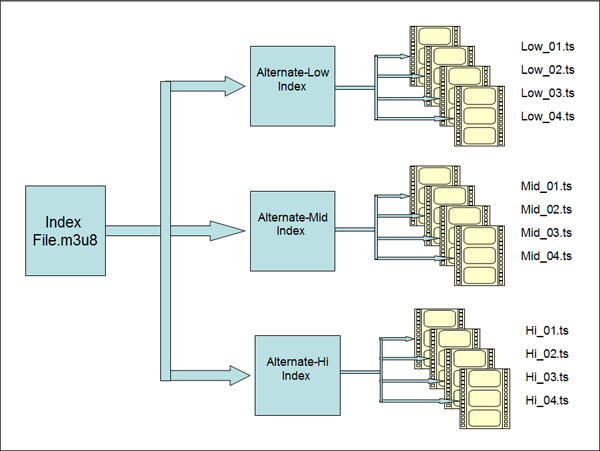
\includegraphics[width=13cm]{img/capitulo_2/hls.jpg}
        \caption{Http Live Streaming.\\}
        Fuente: \cite{hls}
        \label{fig:hls}
    \end{center}
\end{figure}

\subsubsection{DASH}

MPEG DASH (Dynamic Adaptive Streaming over HTTP) es un estándar para la transmisión adaptativa a través de HTTP que tiene el potencial de reemplazar tecnologías patentadas existentes como Microsoft Smooth Streaming, Adobe Dynamic Streaming y Apple HTTP Live Streaming (HLS) \cite{dash_streamingmedia}. Todas las tecnologías de transmisión adaptativa basadas en HTTP utilizan una combinación de archivos multimedia codificados y archivos de manifiesto que identifican transmisiones alternativas y sus respectivas URL.\\

Los reproductores respectivos monitorean el estado del búfer (HLS) y la utilización de la CPU (Smooth Streaming y HTTP Dynamic Streaming) cambiando las transmisiones según sea necesario, ubicando la transmisión alternativa de las URL especificadas en el archivo de manifiesto. HLS usa segmentos MPEG-2 Transport Stream (M2TS), almacenados como miles de pequeños archivos M2TS, mientras que Smooth Streaming y HLS usan código de tiempo para encontrar el fragmento necesario de los flujos elementales MP4 apropiados.\\

En la figura \ref{fig:dash} se visualiza el funcionamiento del estándar DASH. El reproductor realiza las peticiones necesarias a un enlace el cual esta disponible y gestiona las peticiones de los clientes como del servidor en el momente de guardar los videos codificados.\\

\begin{figure}[H]
    \begin{center}
        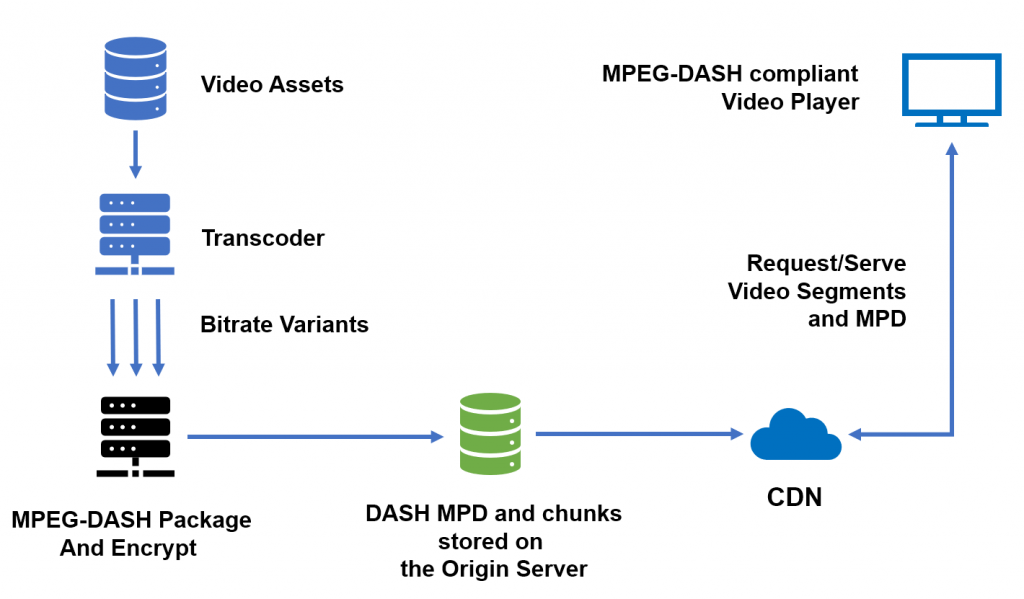
\includegraphics[width=13cm]{img/capitulo_2/dash.png}
        \caption{Dinamyc Adaptative Streamming Over Http.\\}
        Fuente: \cite{dash}
        \label{fig:dash}
    \end{center}
\end{figure}

\section{Lenguaje de Programacion}
Python es un lenguaje de programación interpretado cuya filosofía hace hincapié en la legibilidad de su código. Se trata de un lenguaje multiparadigma, ya que soporta parcialmente la orientación a objetos, programación imperativa y, en menor medida, programación funcional. Es un lenguaje interpretado, dinámico y multiplataforma.\\

\begin{figure}[H]
    \begin{center}
        
\includegraphics[width=1cm]{img/capitulo_2/python.png}
        \caption{Logo del lenguaje de programación Python.\\}
        Fuente: Web
        \label{fig:python}
    \end{center}
\end{figure}

Python usa tipado dinámico y conteo de referencias para la administración de memoria. Una característica importante de Python es la resolución dinámica de nombres; es decir, lo que enlaza un método y un nombre de variable durante la ejecución del programa (también llamado enlace dinámico de métodos). También es usado en el campo del Machine Learning y el Deep Learning. Actualmente es el lenguaje más popular y de ámplio alcance en la inteligencia artificial \cite{python:popular}.\\

\section{Metodología de desarrollo}
El concepto de ingenieria de software es propuesto por primera vez en el conjunto de conferencias históricas organizadas por el comité de ciencia de la OTAN.\footnote{Organización del Tratado del Atlántico Norte.} en los años 60. Para ese tiempo la ingenieria de software tampoco era conocida ni aceptada. En ese entonces los proyectos de software complejos eran problemáticos y costosos de completar, entonces se supuso que sería beneficioso considerar el desarrollo de software como Ingeniería \cite{Ganis}.\\

Los encargados de la codificación del software llamados programadores; en un principio eran ingenieros, pero como el costo computacional era alto, se utilizó un concepto de hardware denominado "mide dos veces, corta una vez"\cite{Ganis}. La naturaleza cautelosa de esta costumbre provocó el desarrollo de metodologías que permitieron a los equipos de proyectos creen planes lentos y metódicos para la creación de sistemas de software.\\

\subsection{Modelo Cascada o Waterfall}
En sus inicios, este concepto fue abordado por el Dr. Winston Royce, por medio de un artículo escrito sobre la gestión y dirección de proyectos grandes y complejos de software \cite{Winston}. En ese artículo en base en experiencias de desarrollo de Software para la planificación de misiones aereas; el autor describe los fundamentos del desarrollo de Software. Gran parte de esos fundamentos aún son aplicables en la actualidad. En el planteamiento de estos fundamentos, Royce presenta un conjunto de fases los cuales forman parte de una secuencia de desarrollo de software ilustrada en la figura \ref{fig:cascada}.\\

\begin{figure}[H]
    \begin{center}
        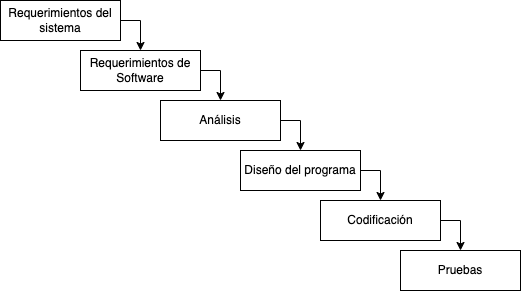
\includegraphics[width=12cm]{img/capitulo_2/cascada2.png}
    \end{center}
    \caption{Modelo Cascada}
    \centering{Fuente: Elaboracion Propia}
    \label{fig:cascada}
\end{figure}

Una vez definida esta secuencia, se crea el concepto de ``Cascada", como un modelo de desarrollo con actividades bien definidas y organizadas con un objetivo independiente dando origen al diseño del primer S.D.M.\footnote{Metodología de Desarrollo de Software} \cite{Bell&Thayer}. En la figura \ref{fig:cascada} la fase de análisis y la de codificación entregan la mayor parte del producto esperado, mientras que las otras fases estan puestas para ser organizadas y planificadas de manera independiente para un mejor manejo de los recursos del proyecto.\\

De acuerdo al modelo Cascada, se enfatiza en la dependecia secuencial del producto entregado en el paso previo. Es decir existe una dependencia que mantiene en espera el diseño del sistema mientras que el análisis del modelo no sea aprobado o concluido y consecuentemente la fase de codificación se verá en espera también hasta que el diseño se concluya.\\

Cada una de las fases guarda una relación iterativa con el siguiente paso definido en la metodología que asegura la completitud del producto entregado en la fase antetior. Esta relación esta ilustrada en la figura \ref{fig:cascada_iterativa}. Al final de cada etapa, el modelo está diseñado para llevar a cabo una revisión final, que se encarga de determinar si el proyecto está listo para avanzar a la siguiente fase. Este modelo fue el primero en originarse y es la base de todos los demás modelos de ciclo de vida dentro de un proyecto de desarrollo de software.\\

En la práctica, se aplican diversas versiones del modelo. Los más habituales son los modelos que dividen los procesos de desarrollo en cinco fases. En ocasiones, las fases 1, 2 y 3 definidas por Royce se integran en una sola fase de proyecto a modo de análisis de los requisitos.\\

\begin{enumerate}
    \item Análisis: planificación, análisis y especificación de los requisitos.
    \item Diseño: diseño y especificación del sistema.
    \item Implementación: programación y pruebas unitarias.
    \item Verificación: integración de sistemas, pruebas de sistema y de integración.
    \item Mantenimiento: entrega, mantenimiento y mejora.
\end{enumerate}

La figura \ref{fig:cascada_iterativa} se muestra la ampliación de esta metodología donde se añaden funciones iterativas al modelo básico como, por ejemplo, los saltos hacia atrás, que permiten comparar los resultados de cada una de las fases con las hipótesis obtenidas en la fase anterior, de modo que se puedan verificar.\\

\begin{figure}[H]
    \begin{center}
        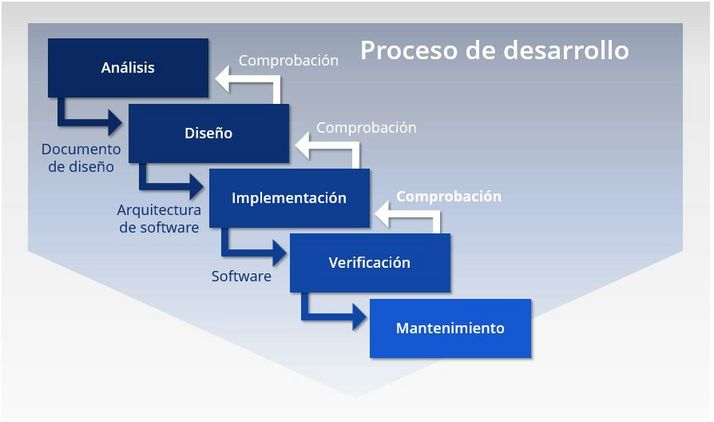
\includegraphics[width=12cm]{img/capitulo_2/waterfall.jpeg}
    \end{center}
    \caption{Modelo Cascada: Relación iterativa entre las fases sucesivas.}
    \centering{Fuente: }
    \label{fig:cascada_iterativa}
\end{figure}

En este modelo, las diferentes fases de un proceso de desarrollo se suceden una detrás de otra como en una cascada. Cada una de las fases concluye con un resultado provisional o ``hito''. A continuacion se detalla cada una de las fases y las actividades que implica cada fase:

\subsubsection{Análisis}

Todo proyecto de software comienza con una fase de análisis que incluye un estudio de viabilidad y una definición de los requisitos. En el estudio de viabilidad se evalúan los costes, la rentabilidad y la factibilidad del proyecto de software. El estudio de viabilidad da como resultado un pliego de condiciones (una descripción general de los requisitos), un plan y una estimación financiera del proyecto, así como una propuesta para el cliente, si fuera necesario.\\

Este es el punto de partida en donde se plasma cada detalle de la idea y tomar el impulso necesario para su desarrollo. Esta fase consiste en determinar cuáles son las necesidades y los objetivos, para luego reunir todos los requisitos que se deben cumplir en el desarrollo del software para llevar a cabo todo el proceso.\\

Se realiza una definición detallada de los requisitos, incluyendo un análisis de la situación de salida y un concepto. Mientras que los análisis de salida se encargan de describir la problemática en sí, el concepto ha de definir qué funciones y características debe ofrecer el producto de software para cumplir con las correspondientes exigencias. La definición de los requisitos da como resultado un pliego de condiciones, una descripción detallada de cómo se han de cumplir los requisitos del proyecto, así como un plan para la prueba de aceptación, entre otros.\\

Por último, la primera fase del modelo cascada incluye un análisis de la definición de los requisitos en el que los problemas complejos se dividen en pequeñas tareas secundarias y se elaboran las correspondientes estrategias de resolución.\\

\subsubsection{Diseño}

La fase de diseño sirve para formular una solución específica en base a las exigencias, tareas y estrategias definidas en la fase anterior. En esta fase, los desarrolladores se encargan de diseñar la arquitectura de software, así como un plan de diseño detallado del mismo, centrándose en componentes concretos, como interfaces, entornos de trabajo o bibliotecas. La fase de diseño da como resultado un borrador preliminar con el plan de diseño del software, así como planes de prueba para los diferentes componentes.\\

\subsubsection{Implementación}

La arquitectura de software concebida en la fase de diseño se ejecuta en la fase de implementación, en la que se incluye la programación del software, la búsqueda de errores y las pruebas unitarias. En la fase de implementación, el proyecto de software se traduce al correspondiente lenguaje de programación. Los diversos componentes se desarrollan por separado, se comprueban a través de las pruebas unitarias y se integran poco a poco en el producto final. La fase de implementación da como resultado un producto de software que se comprueba por primera vez como producto final en la siguiente fase (prueba alfa).\\

\subsubsection{Verificación}
La fase de verificación o pruebas incluye la integración del software en el entorno seleccionado. Por norma general, los productos de software se envían en primer lugar a los usuarios finales seleccionados en versión beta (pruebas beta). Las pruebas de aceptación desarrolladas en la fase de análisis permiten determinar si el software cumple con las exigencias definidas con anterioridad. Aquellos productos de software que superan con éxito las pruebas beta están listos para su lanzamiento.\\

\subsubsection{Mantenimiento}

Una vez que la fase de prueba ha concluido con éxito, se autoriza la aplicación productiva del software. La última fase del modelo en cascada incluye la entrega, el mantenimiento y la mejora del software. En esta fase se analizan los resultados del hito anterior para realizar los cambios pertinentes para dar por concluido el proyecto.\\

\subsection{Ventajas y desventajas del modelo Cascada}
Esta metodología permite estructurar la organización de forma clara en aquellos proyectos de desarrollo en los que las diversas fases de proyecto se diferencian claramente entre sí. Como cada una de las fases concluye con un hito, el proceso de desarrollo es muy fácil de comprender. El punto clave del modelo reside en la documentación de todos y cada uno de los pasos de proceso. Los conocimientos adquiridos se registran en pliegos de requisitos o borradores preliminares.\\

En teoría, el desarrollo en cascada pretende crear los requisitos previos para una ejecución rápida y rentable de los proyectos a través de una cuidada planificación previa. Sin embargo, la utilización del modelo en la práctica es controvertida. Por una parte, en el desarrollo de software las fases de proyecto no suelen estar claramente diferenciadas entre sí.\\

En sentido estricto, el modelo en cascada no prevé la realización de ajustes a lo largo del proyecto. Sin embargo, un proyecto de software en el que todos los detalles del desarrollo se definieran al comienzo, solo podría concluir con éxito si desde el principio se invirtiera una gran cantidad de tiempo y dinero en análisis y diseño.\\

En resúmen se tienen las siguientes ventajas: 
\begin{itemize}
    \item Una estructura sencilla gracias a unas fases de proyecto claramente diferenciadas.
    \item Buena documentación del proceso de desarrollo a través de unos hitos bien definidos.
    \item Los costes y la carga de trabajo se pueden estimar al comenzar el proyecto.
    \item Aquellos proyectos que se estructuran en base al modelo en cascada se pueden representar cronológicamente de forma sencilla.
\end{itemize}

Como también las siguientes desventajas:
\begin{itemize}
    \item  Por norma general, los proyectos más complejos o de varios niveles no permiten su división en fases de proyecto claramente diferenciadas.
    \item Poco margen para realizar ajustes a lo largo del proyecto debido a un cambio en las exigencias.
    \item El usuario final no se integra en el proceso de producción hasta que no termina la programación.
    \item En ocasiones, los fallos solo se detectan una vez finalizado el proceso de desarrollo.
\end{itemize}

Se elige el modelo cascada dado que todas las ventajas se ajustan perfectamente al desarrollo del prototipo de sistemas de video-vigilancia. Por lo tanto las fases que tiene el modelo de desarrollo de software elegido para la realización del proyecto son:

\begin{enumerate}
    \item \textbf{Análisis}: Esta fase se lleva a cabo a través de la definición de requisitos, la planificación y los casos de uso.
    \item \textbf{Diseño}: Esta fase se lleva a cabo mediante un diagrama de secuencia y un diseño de la interfaz.
    \item \textbf{Implementación}: Esta fase se lleva a cabo mediante la implementación del Sistema de video-vigilancia inteligente.
    \item \textbf{Pruebas}: Esta fase se lleva a cabo mediante la realización de pruebas sobre el sistema de video-vigilancia.
\end{enumerate}
